\contourlength{1.0pt}
\tikzset{>=latex} % for LaTeX arrow head

\colorlet{xcol}{blue!60!black}
\colorlet{myred}{red!80!black}
\colorlet{myblue}{blue!80!black}
\colorlet{mygreen}{green!40!black}
\colorlet{myorange}{orange!90!black}
\colorlet{mypurple}{red!50!blue!90!black!80}
\colorlet{mydarkred}{myred!80!black}
\colorlet{mydarkblue}{myblue!80!black}
\tikzstyle{xline}=[xcol,thick]
\tikzstyle{width}=[{Latex[length=5,width=3]}-{Latex[length=5,width=3]},thick]
\tikzset{
  traj/.style 2 args={xline,postaction={decorate},decoration={markings,
    mark=at position #1 with {\arrow{<}},
    mark=at position #2 with {\arrow{<}}}
  }
}
\def\tick#1#2{\draw[thick] (#1)++(#2:0.12) --++ (#2-180:0.24)}
\def\N{100} % number of samples

% CIRCLE on axis




% COS
\def\xmax{6.6} % max x axis
\def\ymax{1.2} % max y axis
\def\A{0.8}    % amplitude
\def\om{(2.55*360/(0.94*\xmax))} % angular frequency in degrees


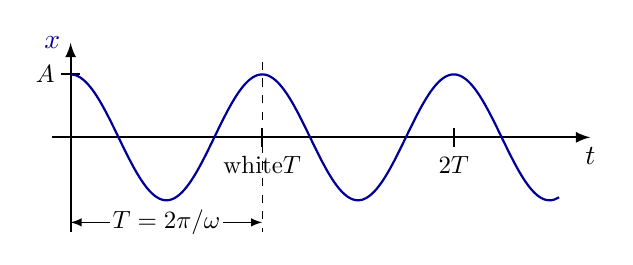
\begin{tikzpicture}
  
  % AXIS
  \draw[->,thick] (0,-\ymax) -- (0,\ymax) node[left,xcol] {$x$};
  \draw[->,thick] (-0.2*\ymax,0) -- (\xmax,0) node[below] {$t$};
  \draw[dashed] ({360/\om},1.2*\A) --++ (0,-2.7*\A);
  \tick{0,\A}{0} node[left=-1,scale=0.9] {$A$};
  \tick{{360/\om},0}{90} node[below,scale=0.9] {\contour{white}{$T$}};
  \tick{{720/\om},0}{90} node[below,scale=0.9] {$2T$};
  \draw[<->]
    (0,-1.35*\A) --++ ({360/\om},0)
    node[midway,fill=white,inner sep=1,scale=0.9] {$T = 2\pi/\omega$};
  
  % PLOT
  \draw[xline,samples=\N,smooth,variable=\x,domain=0:0.94*\xmax]
    plot(\x,{\A*cos(\om*\x)});
  %\node[xcol,above=2,right=4] at ({720/\om},\A) {$x(t)=A\cos(\omega t)$};
  
\end{tikzpicture}
